\documentclass{article}

% Language setting
% Replace `english' with e.g. `spanish' to change the document language
\usepackage[english]{babel}

% for autocsv
\usepackage{csvsimple}

% Set page size and margins
% Replace `letterpaper' with `a4paper' for UK/EU standard size
\usepackage[letterpaper,top=2cm,bottom=2cm,left=3cm,right=3cm,marginparwidth=1.75cm]{geometry}

% Useful packages
\usepackage{amsmath}
\usepackage{graphicx}
\usepackage[colorlinks=true, allcolors=blue]{hyperref}

\graphicspath{ {./images/} }

\setlength{\parindent}{0pt}

\title{Modeling COVID-19 Outcomes: Predictive Insights into Deaths, Hospitalizations, and ICU Admissions}
\author{CID 1843091}

\date{May 2024}

\begin{document}
\maketitle

\section{Introduction}

The global COVID-19 pandemic has posed unprecedented challenges to healthcare systems worldwide, highlighting the critical need for accurate predictive models to forecast key outcomes such as deaths, hospitalizations, and ICU admissions. The motivation for this research stems from the urgent demand for reliable tools that can anticipate the trajectory of the pandemic and inform decision-making at various levels, from governmental authorities to healthcare providers and policymakers.\\

Our project looks at the \href{https://github.com/owid/covid-19-data}{OWID COVID-19 dataset} and aims to model the number of deaths, hospitalizations and ICU admissions as a function of other predictors.

\section{Dataset Exploration}

\subsection{Choice of variables}

We are specifically interested in 3 responses in the dataset:

\begin{enumerate}
\item new deaths smoothed per million
\item weekly icu admissions per million
\item weekly hosp admissions per million
\end{enumerate}

These response variables were chosen because they were invariant to the population size of the country (unlike say new deaths) and they are assumed to be stationary in time (unlike say total deaths). It should also be noted they are smoothed by taking a 7 day average to account for reporting practices of the figures. For example, some countries only report their figures once a week which would make the counts on other days of the week 0. This is undesirable because it makes the data irregular and introduces unnecessary structure to the data for the model to learn. \\

The dataset in question records a large number of variables as possible predictors we can use and ideally we would like to use all of them as predictors and look at which predictors are the most important/impactful in predicting the response. However a brief look at the dataset and we can see many entries are NaN. There are 2 possible reasons for this:

\begin{enumerate}
\item Some countries do not record the data at all
\item Some countries did not record the data in the period before because it was not relevant
\end{enumerate}

An example for the second reason is at the beginning of the pandemic (around 2020 Jan) there was no testing for COVID-19 in many countries because it was not yet well known and hence many entries for total cases are NaN. However as it became more well known (or severe), recording and reporting these figures began.\\

We would first like to filter out countries that do not record the 3 response variables we are interested in to look at the size of the dataset available to us. Doing so, we got 21 countries which all recorded out responses at some points in time, their ISO codes are as follows:\\

'CHL', 'CYP', 'CZE', 'DEU', 'ESP', 'EST', 'FRA', 'GRC', 'HUN', 'IRL', 'ISR', 'ITA', 'KOR', 'LUX', 'LVA', 'MLT', 'NLD', 'NOR', 'SGP', 'SVK', 'SVN'

We then looked at the set of predictor variables available in the dataset that were recorded by all 21 countries above with the additional criteria of choosing the statistics that were invariant to population size and stationary. We separate our predictors into 2 kinds, time dependent predictors and 'constant' predictors. Our time dependent predictors were:\\

'people fully vaccinated per hundred', 'new cases smoothed per million', 'tests per case', 'new vaccinations smoothed per million', 'stringency index'\\

Our constant predictors were:\\

'population density', 'median age', 'aged 65 older', 'aged 70 older', 'gdp per capita', 'cardiovasc death rate', 'diabetes prevalence', 'male smokers', 'female smokers', 'hospital beds per thousand', 'life expectancy', 'human development index'\\

Note that technically speaking these values should fluctuate over time but these changes occur over long time frames like decades, so for purposes of the dataset and our paper we will assume they are constant.

\subsection{Heatmap of variables}

After cleaning the data it helps to look at the rough distribution/scale of the data to either make model design choices or clean it further. We plot the heatmaps (Fig \ref{fig:heat1} and \ref{fig:heat2}) of the predictors and response to do this:

\begin{figure}
\centering
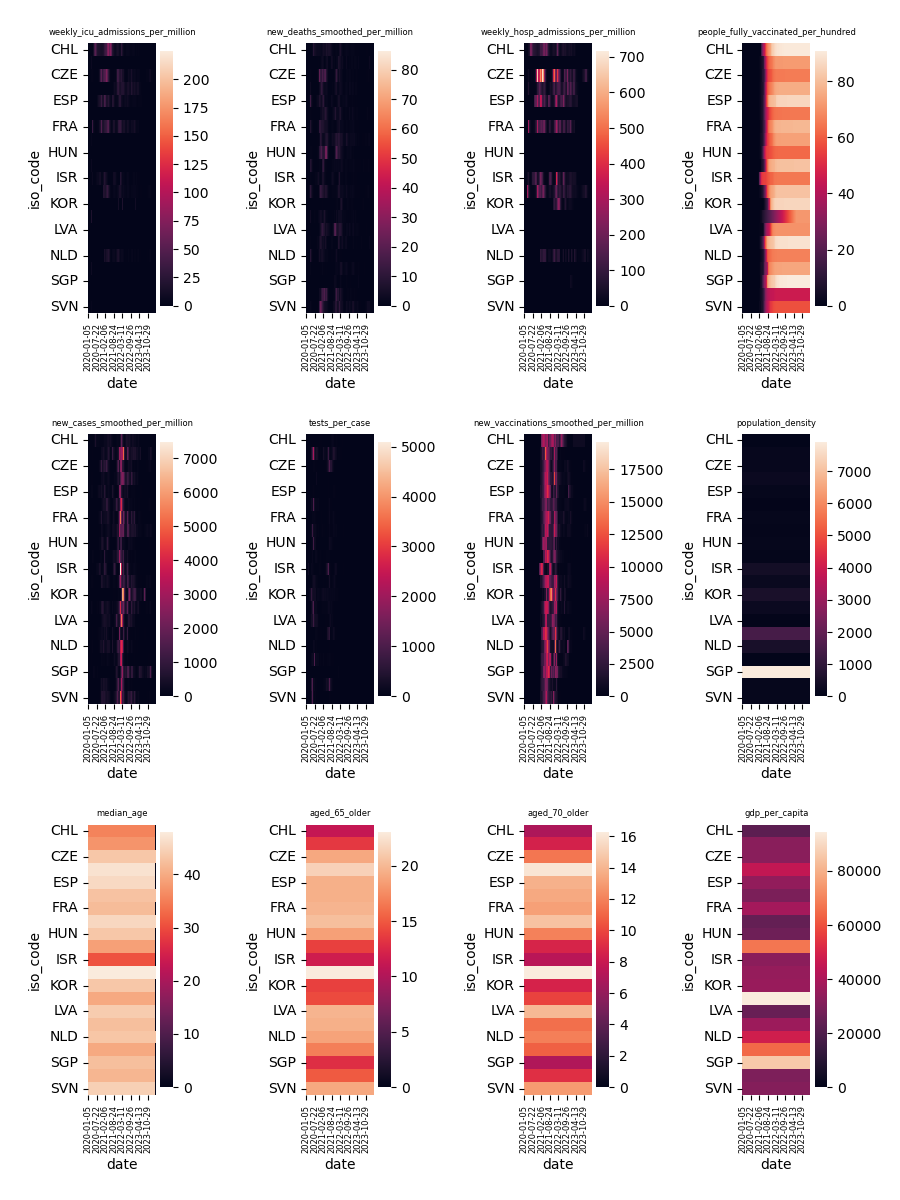
\includegraphics[width=1\linewidth]{heatmap_plot1.png}
\caption{\label{fig:heat1}Heatmap 1 of predictors and response}
\end{figure}

\begin{figure}
\centering
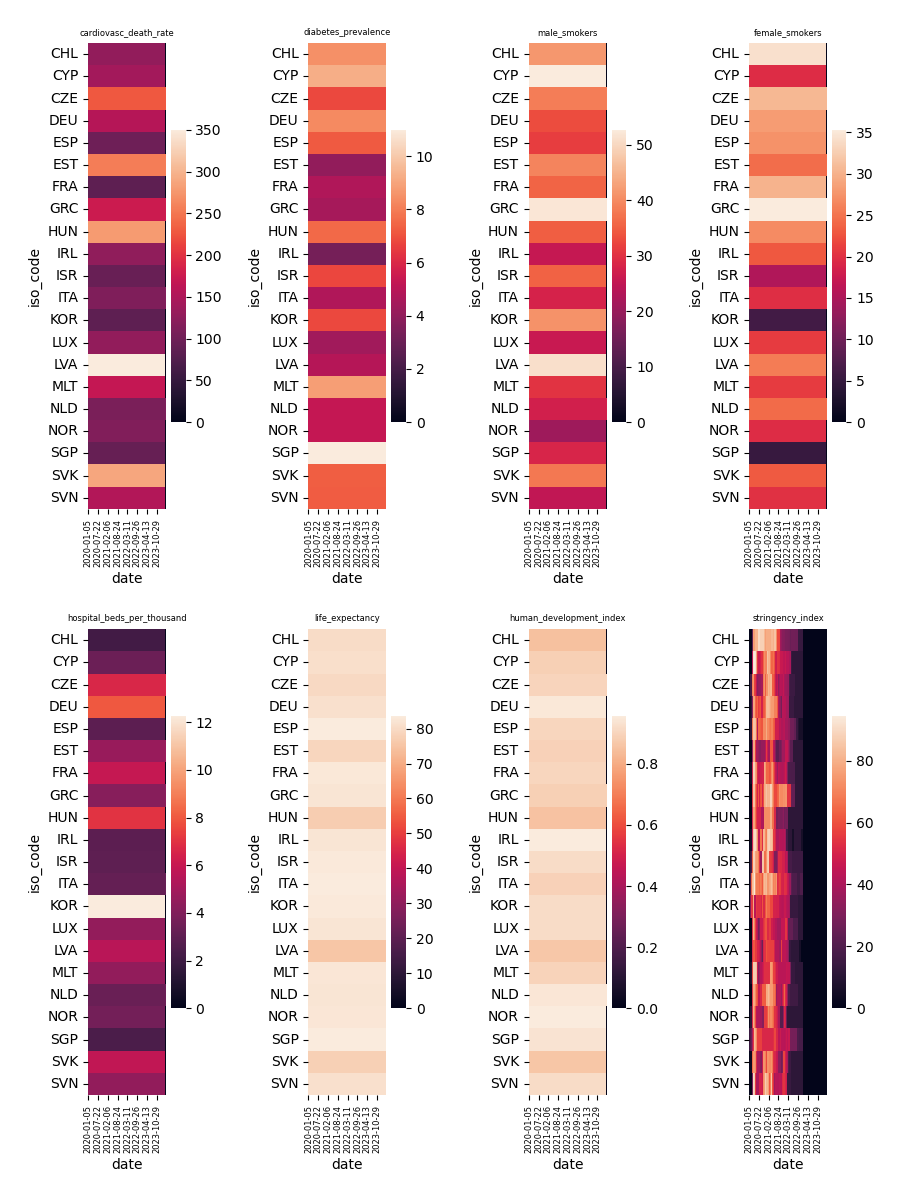
\includegraphics[width=1\linewidth]{heatmap_plot2.png}
\caption{\label{fig:heat2}Heatmap 2 of predictors and response}
\end{figure}

\clearpage 

\subsection{ACF and PACF}

One possible common model is the ARIMA model and we would like to evaluate how suitable of the model is and if so what parameters should be used. Typically this involves checking if the time series is stationary and plotting the ACF and PACF plots.\\

\begin{table}
\csvautotabular{tables/adfstat.csv}
\caption{\label{tab:adf}ADF Statistic Test for Stationary}
\end{table}

In Table \ref{tab:adf}, we see the p-values of the ADF statistic test which tests the null hypothesis that a unit root is present in a time series sample. We see that the p-values are low, across all ISO codes and responses which suggest that they are stationary (reject the null hypothesis that a unit root is present). \\

We look at the ACF and PACF plots (up to lag 15) of the three variables of a randomly chosen ISO code ('SGP') in Fig \ref{fig:acf}. This is not promising since we see 0 correlation for all lags which suggest that an ARIMA model is unsuitable for modelling the responses.\\

\begin{figure}
\centering
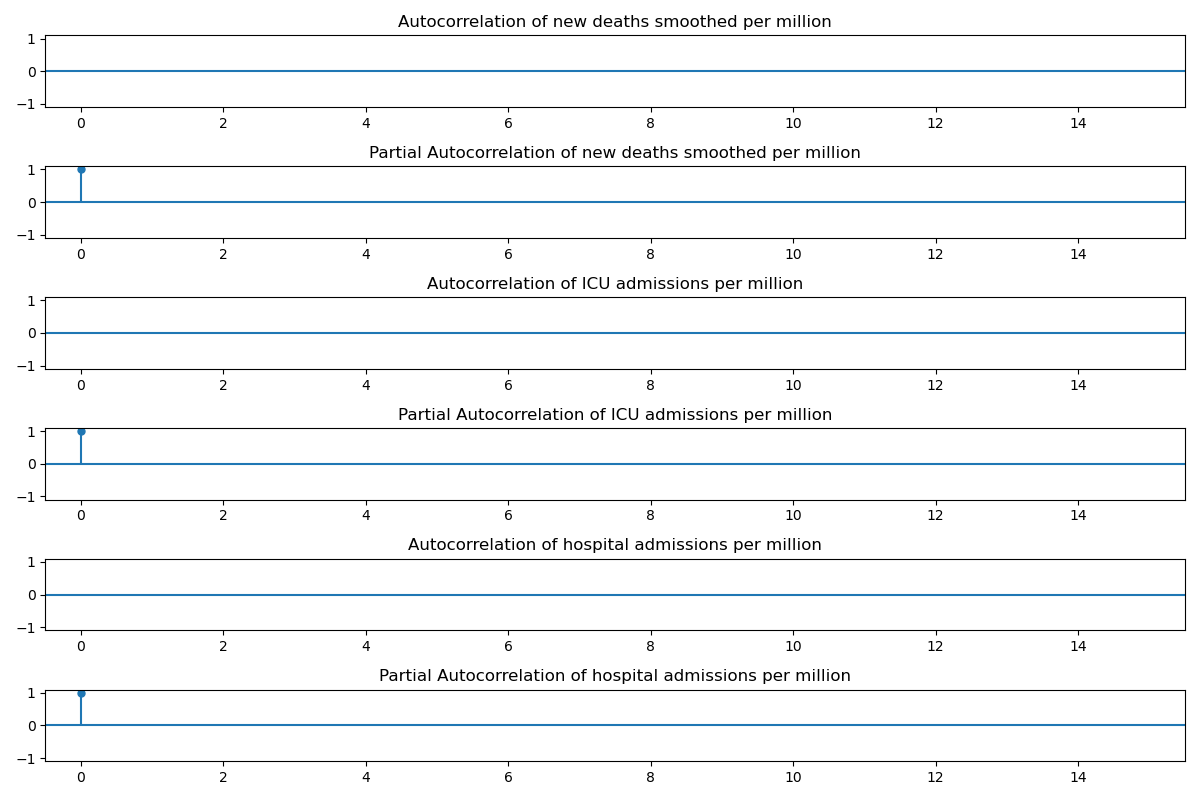
\includegraphics[width=1\linewidth]{acf.png}
\caption{\label{fig:acf}ACF and PACF plots of response variables for SGP}
\end{figure}

\clearpage

\section{Methodology}


Our main goal is to predict the response $y_t$ as a function of previous data, $y_{t-1}, x_{t-1}, y_{t-2}, x_{t-2},...$ where $x$ are the predictors mentioned earlier. It's not clear how far back in time we should look back so in general this is one of the hyperparameters we will vary for all models. We will look at 3 main models  in increasing degree of complexity (but at cost of model interpretability):

\begin{enumerate}
\item Linear Model with varying regularisation
\item Random Forest Model with varying depth
\item Multi-Layer Perceptron with varying architecture
\end{enumerate}

In general our hyperparameters will be selected by grid search. We will first split the data into train/validation and test sets. The train/validation sets will be used by the 3 models to train and do hyperparameter tuning. The test set will be reserved exclusively for evaluating the final 3 models.\\

\subsection{Splitting Time Series Data}

Unlike non time series data, splitting the data into train and test sets is not a straightforward procedure of shuffling and taking data points. The reason is that time series data may contain information about the past. This is problematic since if we train our model on future data and evaluate on past data, there may be data leakage. As such train-test(or validation) splits need to respect chronological order. \\

There are 2 ways we can split train and test sets:

\begin{enumerate}
\item We can split by countries and train our data that way
\item We can split by time and train our data that way
\end{enumerate}

In our opinion, using the first method is problematic  since often the different country data is correlated (for the same time period). This is problematic since it may just cause data leakage from the test set. As such we use the second method, splitting our train and test sets by time. We first split the data (chronologically) into train and test sets with a $0.9$-$0.1$ ratio. 

\subsection{Walk Forward Validation}

Typically cross validation is employed to get a more robust measure of the performance of a model (for a chosen hyperparameter choice), but as discussed above this is problematic for time series data. Hence we employ walk forward validation where we split the data into chronological blocks  (say $B_1, B_2, ..., B_{n+1}$). To conduct walk forward validation, at split $i$ (where the total number of split is $n$), we train on $\cup_{j\leq i}B_j$ (of all the countries) and validate on $B_{i+1}$. 

\subsection{Loss and Score}

For purposes of training our models we will use Mean Squared Error (MSE), but we will often compare or compute the $R^2$ score which is $\left(1 -\frac{\sum (y_i - \hat{y}_i)^2}{\sum (y_i - \bar{y})^2}\right)$. Note that maximising $R^2$ score is equivalent to minimising MSE loss so in terms of optimisation they are equivalent. We compute the $R^2$ score because it is invariant under the affine transformations and provides a good benchmark where the best possible score is 1 and a score of 0 is equivalent to a model which just predicts the mean $\bar{y}$

\subsection{Rescaling Data}

We saw in Fig \ref{fig:heat1} and \ref{fig:heat2} that the values range over a wide scale and also some variables tend to be sparse. This makes normalising variables to 0 mean and 1 std problematic. So we rescale all variables to be in the interval $[0,1]$ (Note that we fit only on the train/validation  set and do not use the test set to avoid data leakage).

\section{Linear Model}

For the Linear model, we look at the following hyperparameters:

\begin{enumerate}
\item Regularisation type: L1(LASSO), L2(Ridge) 
\item Magnitude of regularisation: $10^{-4}, 10^{-3}, 10^{-2}, 10^{-1}, 10^{0}, 10^{1}, 10^{2}$
\item Number of days in the past to look at (we term as shift): $1, 2, 3, ..., 10$
\end{enumerate}

Note that in the above if shift is $3$, the we model $y_t = f(x_{t-1},x_{t-2},x_{t-3}, y_{t-1},y_{t-2},y_{t-3})$ where $f$ is an affine transformation above. 

\begin{figure}
\centering
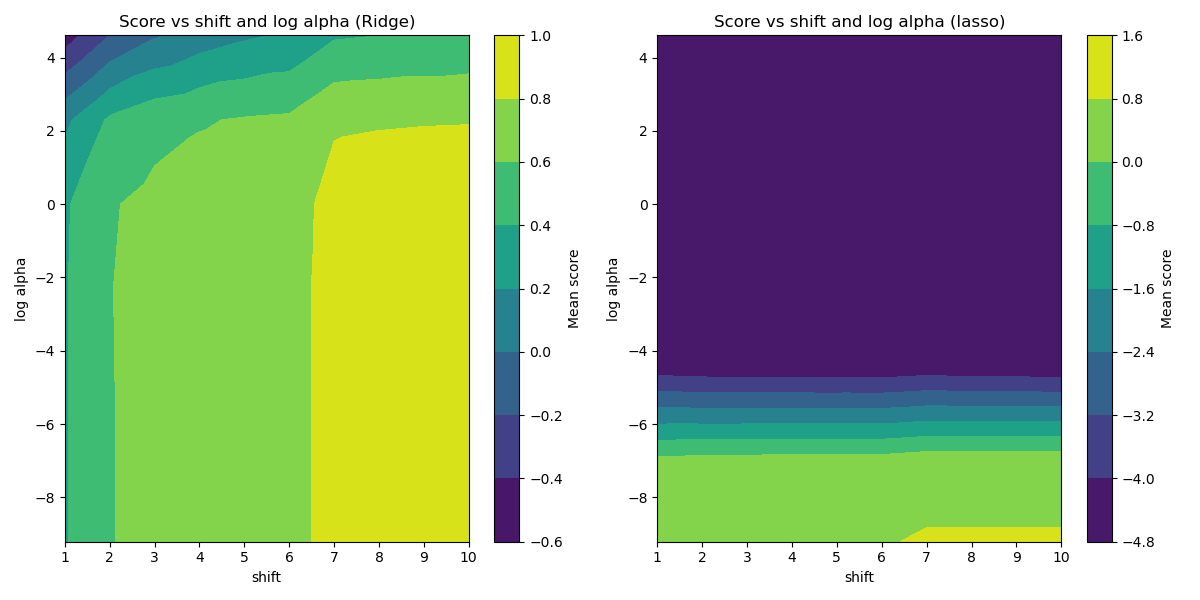
\includegraphics[width=1\linewidth]{lm_plot.png}
\caption{\label{fig:lm}Contour plot of score of different hyperparameters of Linear model}
\end{figure}

Our best performing set of hyperparameters is Ridge linear model with $10^{-3}$ regularisation magnitude and 10 shift with a validation score of 0.93.

\section{Random forest}

For the random forest model, we look at the following hyperparameters:

\begin{enumerate}
\item Bootstrap or non-Bootstrap samples
\item Maximum depth of tree: $5, 10, 20, 40,$ None
\item Number of days in the past to look at (we term as shift): $1, 2, 3, ..., 10$
\end{enumerate}

Note that in the above None maximum depth means there is no limit on maximum depth of the tree.

\begin{figure}
\centering
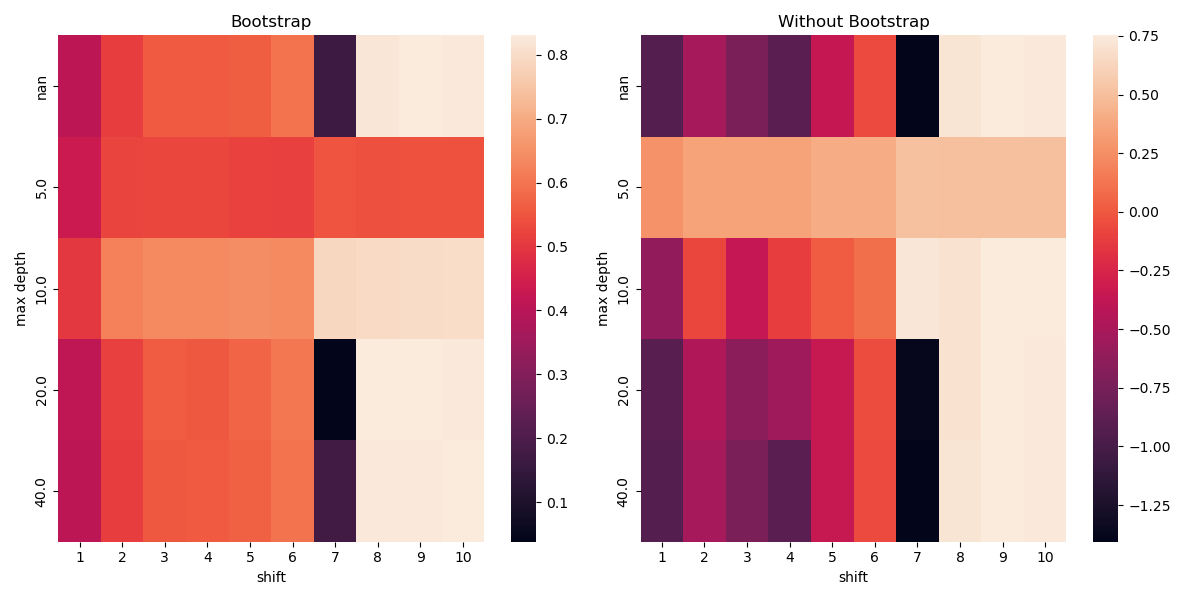
\includegraphics[width=1\linewidth]{rf_plot.png}
\caption{\label{fig:rf}Heat plot of score of different hyperparameters of Random Forest model}
\end{figure}

Our best performing set of hyperparameters is Bootstrapped Random Forest model with $40$ depth and 10 shift with a validation score of 0.83.

\clearpage

\section{Neural Network (MLP)}

Note that unlike the previous 2 models, neural networks are sensitive to feature scales, hence we need to standardize/normalize the data. From the previous heatmap we note that some data like new deaths are sparse (many zeros), this will make normalization problematic. Hence we decide to scale it to min 0 max 1 (and not variance normalization). We fit the scaler to the train/validation set to prevent data leakage.

Due to long training times, we do no carry out walk forward validation while training our MLP model. Instead we fix a training and validation split (again respecting chronological split). We look at the following hyperparameters:

\begin{enumerate}
\item Number of hidden layers: $1, 2, 3$
\item Number of units per layer: $256, 512, 1024$
\item Number of days in the past to look at (we term as shift): $1, 5, 10$
\end{enumerate}

For the architecture we used 0.1 dropout with ReLU activation for the hidden layers and sigmoid activation for the final layer (with 3 units). We trained it with early stopping patience of 5 epochs (looking at validation loss) up to a maximum of 50 epochs, and saved the epoch with the best validation loss as the best weights trained for a chosen set of hyperparameters. 

Due to long training time, we had to settle for a smaller choice of hyperparameters which restricted our choices. 

Our best performing set of hyperparameters is 1 hidden layers with $256$ unit per layer and 10 shift with a validation score of -0.189. 

\clearpage

\section{Evaluating on Test Set}

Finally, we take the best set of hyperparameters of each model, train it on the whole train/validation set and then evaluate the performance on the test set. From the validation scores we saw earlier we would expect the Linear Model to perform the best but in fact from Table \ref{tab:testscore} the Random forest model performed the best when evaluating the Test set although the performance is close\\

In general, we note that increasing the number of days we look back at (shift) increases model performance. This suggests that information as far back as 10 days were helpful in predicting the response. We also further note that test scores were better than in validation. This might be because we trained the final models on the full train/validation set and not the smaller slices previously.

\begin{table}
\csvautotabular{tables/test_scores.csv}
\caption{\label{tab:testscore}Validation and Test Scores for best hyperparameters for 3 models}
\end{table}

\section{Conclusions and Future Work}

In general the models we trained performed quite well with $>0.9 R^2$ score for test evaluation. Due to time and computation constraints, the architecture and choice of hyperparameters for searching were small. Further work on more complicated Neural Networks architecture or more extensive hyperparameter tuning will be interesting to consider. 

\clearpage

\end{document}